\documentclass{article}
\usepackage{tikz}

\begin{document}
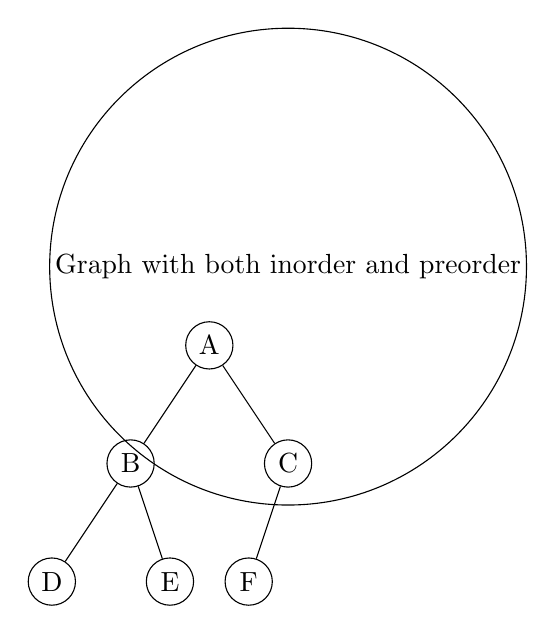
\begin{tikzpicture}[every node/.style={circle, draw, inner sep=2pt, minimum size=6mm}]
    \node (A) at (0,0) {A};
    \node (B) at (-1,-1.5) {B};
    \node (C) at (1,-1.5) {C};
    \node (D) at (-2,-3) {D};
    \node (E) at (-0.5,-3) {E};
    \node (F) at (0.5,-3) {F};
    
    \draw (A) -- (B);
    \draw (A) -- (C);
    \draw (B) -- (D);
    \draw (B) -- (E);
    \draw (C) -- (F);
    \node [draw] at (1,1) {Graph with both inorder and preorder};
\end{tikzpicture}
\\
\begin{tikzpicture}[every node/.style={circle, draw, inner sep=2pt, minimum size=6mm}]     
    \node (A) at (0,0) {A};
     \node (B) at (-1,-1.5) {B};
     \node (C) at (-4,-6) {C};
     \node (D) at (-2,-3) {D};
     \node (E) at (-3,-4.5) {E};
     \node (F) at (-5,-7.5) {F};
                  
     \draw (A) -- (B);
     \draw (B) -- (D);
     \draw (D) -- (E);
     \draw (E) -- (C);
     \draw (C) -- (F);
 \end{tikzpicture}       

\end{document}

